\documentclass{article}

\usepackage{url} 

\usepackage{pdfpages}
\usepackage{lastpage}
\usepackage{fancyhdr}
\usepackage{ngerman}
\usepackage{listings}

\usepackage{floatrow}
\usepackage[tableposition=top]{caption}
\floatsetup[table]{capposition=top}

\usepackage{amsmath, amssymb}

\usepackage[utf8]{inputenc}


\usepackage[numbib]{tocbibind}



\newcommand\twodigits[1]{%
   \ifnum#1<10 0#1\else #1\fi
}



\lhead{Oszillograph}
\rhead{16. Oktober 2020\\T. Maier, J. Winkler}
%\cfoot{\twodigits{\thepage}~/ \pageref{LastPage}}
\cfoot{{\thepage}~/ \pageref{LastPage}}

\newcommand{\as}{\alpha_\text{spez}}

\begin{document}

\parindent0cm

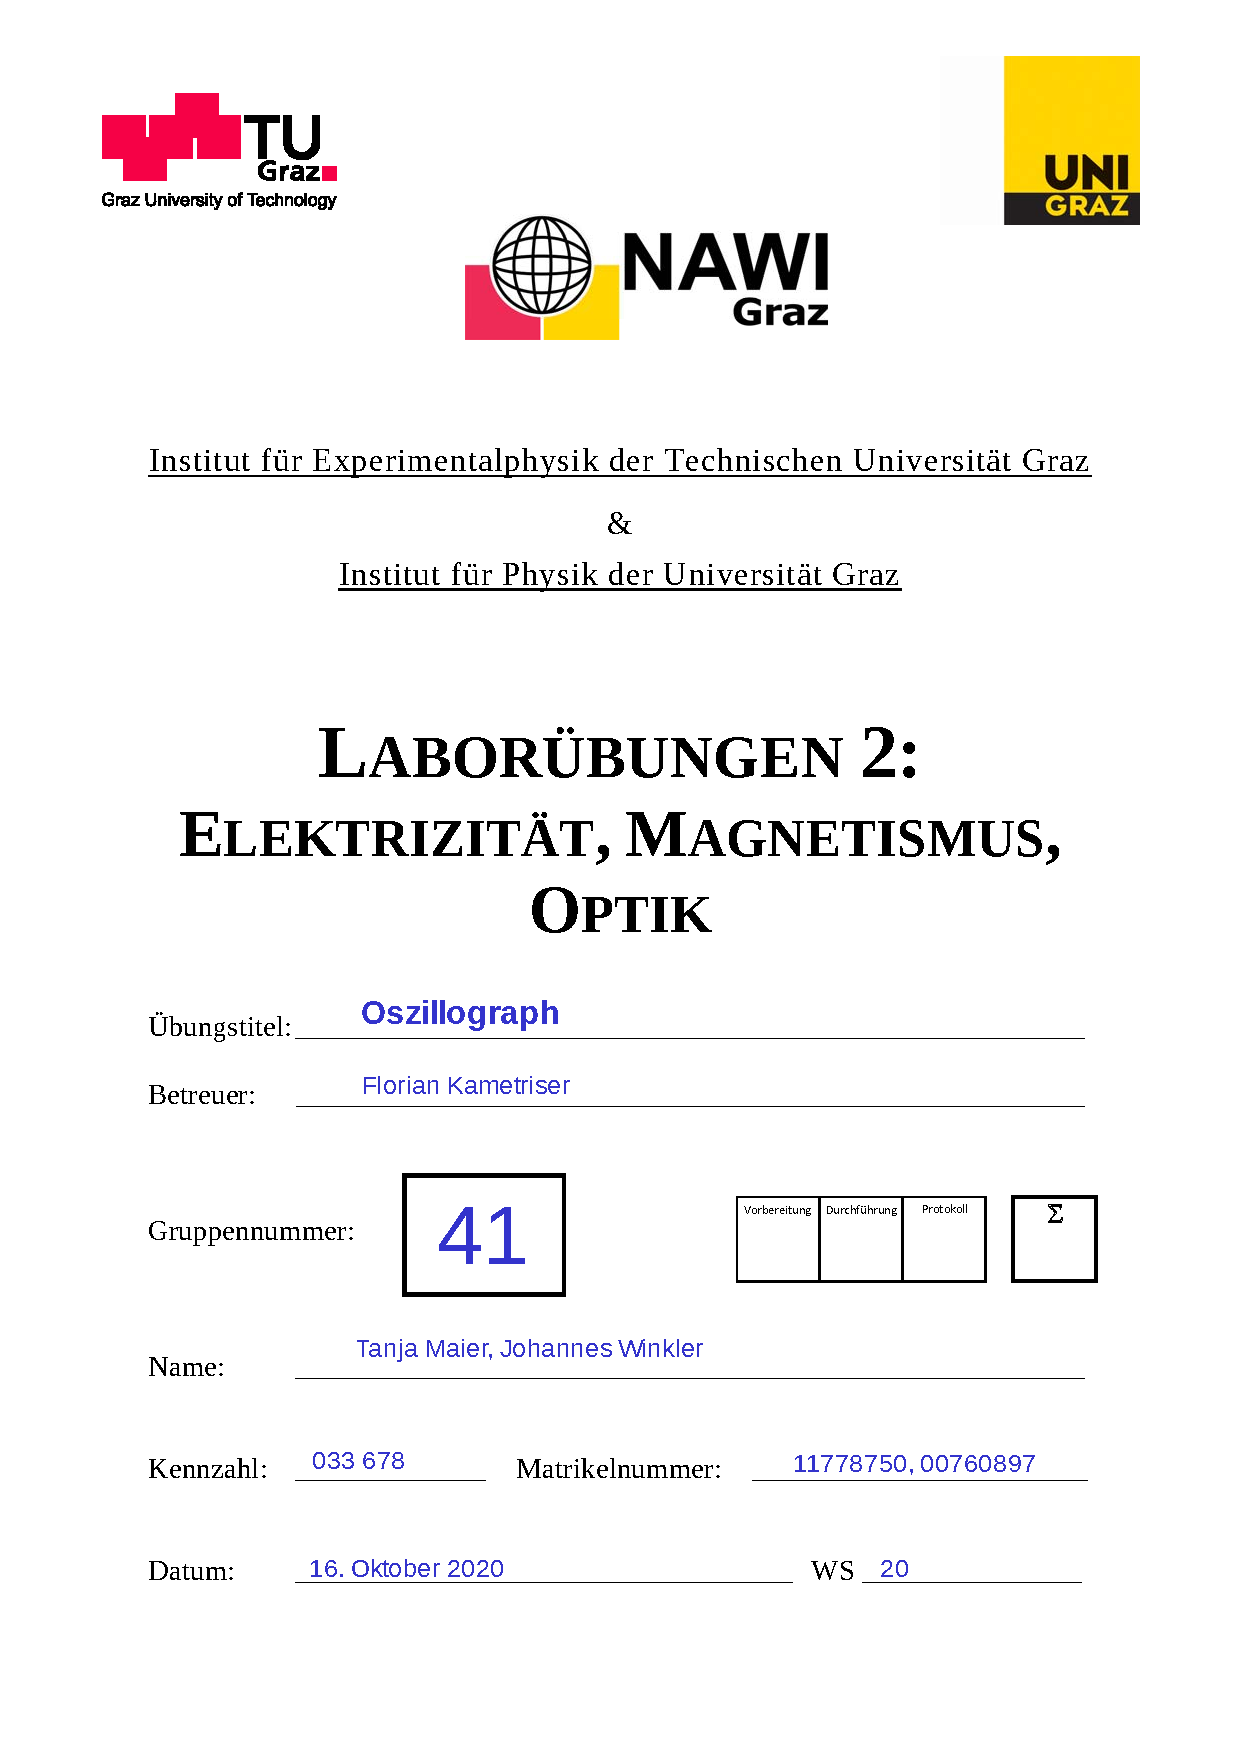
\includepdf{Deckblatt.pdf}


\pagestyle{fancy}

\section{Aufgabenstellung}

Es sind 2 Schaltungen aufzubauen und die dazugehörigen Spannungsverläufe sind zu messen.

\begin{enumerate}
\item Eine RC-Schaltung mit $R=1$~k$\Omega$ und $C=1~\mu$F bei  einer Frequenz mit $f=50~$Hz, wobei einmal eine Sinus- und einmal eine Rechtecksfrequenz angewendet wird.

\item eine RLC-Schaltung mit $R=1$~k$\Omega$ bzw. $R=200~\Omega$ und $C=1~\mu$F und variabler Induktivität. Zusätzlich müssen durch variieren der Induktivität folgende Fälle dargestellt werden. Die Frequenz beträgt erneut $f=50~$Hz.
\begin{enumerate}
\item Schwingfal
\item Kriechfall
\item aperiodischer Grenzfall
\end{enumerate}
\end{enumerate}




\section{Grundlagen}

\subsection{Oszilloskop}

Ein Oszilloskop ist ein Gerät aus der Elektronik, mit dem man Spannungsschwankungen innerhalb zeitlicher Abläufe messen kann. Auf der $x$-Achse ist dabei die Zeit und auf der $y$-Achse die jeweilige Spannung abzulesen.

Das Prinzip dahinter ist auf die Bewegung von Teilchen in einem elektrischen Feld und somit auf die Braun'sche Röhre zurückzuführen.

Bei der Braun'schen Röhre (= Kathodenstrahlröhre) kann durch zwei parallel ausgerichtete Metallplatten Elektronenstrahl quer zu seiner Flugrichtung beeinflusst werden. Die Elektronen werden von der Kathode emittiert und durch eine angelegte Spannung zur Anode $A$ hin beschleunigt.

Um den Strahl zu fokussieren werden zwei elektrische Linse $F$ und die angelegte Fokussierspannung $U_F$ genutzt.


Zur Ablenkung des Elektronenstrahls werden dann vier weitere Platten nach der Anode angebracht. Diese werden zu zweit platziert und mit einer horizontalen Kippspannung ($U_x$) bzw. einer vertikalen Messspannung ($U_y$) versehen. Damit werden die Elektronen abgelenkt und treffen auf den Leuchtschirm am Ende der Röhre.

Mithilfe der Spannung zwischen Kathode K und Wehnelt-Zylinder WZ kann dann noch die Helligkeit des am Schirm abgebildeten Leuchtpunktes variiert werden. \cite{braun} \cite{uniunterlagen}

\subsection{RLC-Stromkreis}

Ein RLC-Stromkreis besteht aus einem Kondensator mit der Kapazität $C$, einer Spule mit Induktivität $L$ und einem Widerstand mit der Größe $R$. Alle Bauteile sind hierfür in Reihe geschalten und somit gilt die Kirchhoff'sche Maschenregel
\begin{align}
\label{eq:maschen}
U_C + U_L + U_R = 0
\end{align}

$U_C$ ist dabei die Spannung am Kondensator, $u_L$ die Spannung an der Spule und $u_R$ die Spannung am Widerstand. Durch Ersetzen von 
\begin{align*}
U_L &= L \cdot \frac{dI}{dt} \\
U_R &= R_i \cdot I
\end{align*}
sowie differenzieren der Formel \eqref{eq:maschen} und ersetzen von 
\begin{align*}
I = i_C = C \cdot \frac{dU}{dt}
\end{align*}
 erhält man die Differentialgleichung des Schwingkreises
\begin{align}
\frac{d^2I}{dt^2} + \frac{R}{L}\cdot \frac{dI}{dt} + \frac{1}{L\cdot C}\cdot I = 0
\end{align}
Durch Lösung dieser Differentialgleichng ergeben sich im wesentlichen 3 mögliche Fälle
\begin{enumerate}
\item $R^2\cdot C - 4\cdot L > 0$: 2 reelle Lösungen, Kriechfall
\item $R^2\cdot C - 4\cdot L = 0$: 1 reelle Lösung, aperiodischer Grenzfall
\item $R^2\cdot C - 4\cdot L < 0$: 2 konjugiert-komplexe Lösungen, Schwingfall
\end{enumerate}



\section{Versuchsaufbau}

\begin{figure}[H]
\caption{Versuchsaufbau der RC-Schaltung. $F$ Frequenzgenerator, $T$ Trenntrafo, $R$ Widerstand, $C$ Kondensator.}
\label{fig:schaltung1}
{\centering
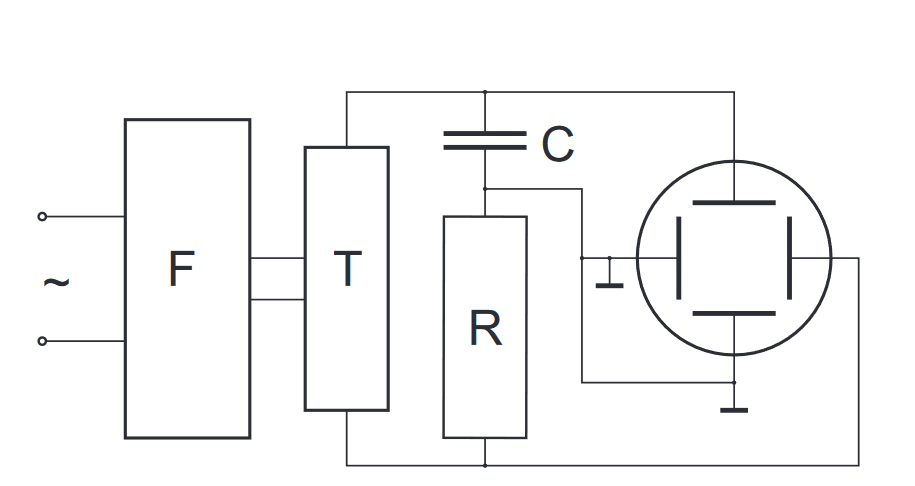
\includegraphics[scale=0.4]{basics1.png}}
\end{figure}

\begin{figure}[H]
\caption{Versuchsaufbau der RLC-Schaltung.}
\label{fig:schaltung2}
{\centering
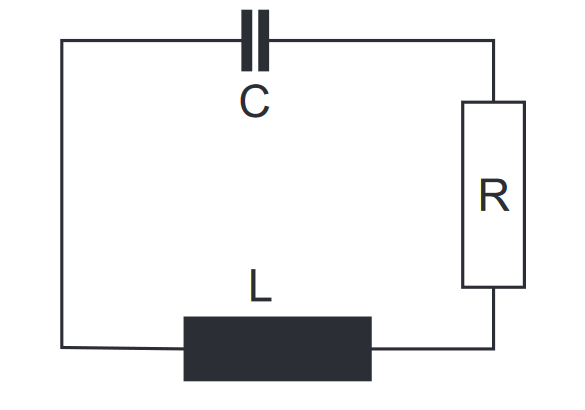
\includegraphics[scale=0.4]{basics2.png}}
\end{figure}


\section{Geräteliste}

\begin{table}[H]
\caption{Liste der verwendeten Geräte}

~

\begin{tabular}{l|llll}
Bezeichnung & Hersteller & Gerätenummer & Unsicherheit \\
\hline
Frequenzgenerator & Wavetek & 0161674  \\
Trenntransformator & \\
Oszilloskop & RIGOL &DS1ET204711289 \\
Widerstand $1$~k$\Omega$ & Rosenthal & & $\pm~1\%$ \\
Widerstand $200~\Omega$ & Rosenthal & & $\pm~1\%$ \\
2x Spule $n=500$ & & 843/3 \\
Kondensator $1~\mu$F & Philips
\end{tabular}

\end{table}




\section{Durchführung und Messwerte}

\subsection{RC-Schaltung}

Ein in Serie geschalteter Kondensator $C$ und ein Widerstand $R$ werden mit einem Frequenzgenerator verbunden. Um einen Kurzschluss über die Erdung und die dadurch resultierende Schädigung der Bauteile zu vermeiden, wird zwischen Frequenzgenerator und den Bauteilen noch ein Trenntrafo geschalten. Der Frequenzgenerator wird auf eine konstante Frequenz von $f=50~$Hz geschalten, wobei einmal eine Rechtecksspannung und einmal eine Sinusspannung angelegt wird. Die Spannungsverläufe über Kondensator und Widerstand werden mit dem Oszilloskop gemessen. Der Versuchsaufbau ist in Grafik \ref{fig:schaltung1} beschrieben.


\subsection{RLC-Schwingkreis}

In die gegebene Schaltung werden zwei seriell geschaltene Spulen mit jeweils $n=500$ Windungen eingefügt. Dadurch wird aus der RC-Schaltung ein Schwingkreis. Der Versuchsaufbau ist in Grafik \ref{fig:schaltung2} beschrieben.

\section{Auswertung}

\subsection{RC-Schaltung}

Die Spannungsverläufe über Kondensator und Widerstand sind in Grafik \ref{fig:schaltung1_sinus} beschrieben. Da Spannung und Strom in einem Widerstand proportional sind, kann anhand der Grafik auch die Phasenverschiebung bestimmen.


\begin{figure}[H]
\caption{Spannungsverläufe einer RC Schaltung mit $R=1~$k$\Omega$ und $C=1\mu~$F bei einer Sinusfrequenz mit $f=50~$Hz. Channel 1 ist die Spannung über den Widerstand, Channel 2 ist die Spannung über den Kondensator. Channel 2 ist um den Faktor 4 vertikal skaliert.}
\label{fig:schaltung1_sinus}
{\centering
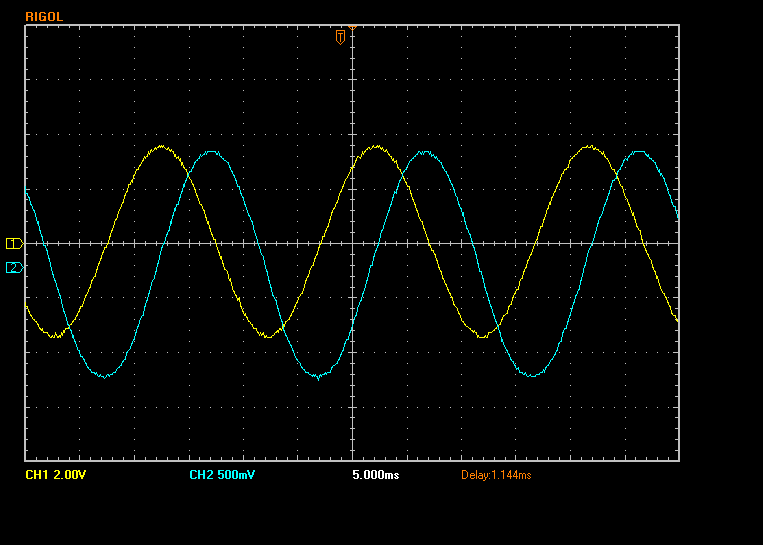
\includegraphics[scale=0.4]{winkler/Schaltung_1_Sinus.png}}
\end{figure}




\subsubsection{Periodendauer}
Hier kann aus den Daten verschiedene Eigenschaften der Schaltung ermitteln. Aus den $f=50~$Hz folgt, dass die Periodendasuer $\tau = 20~$ms sein muss. Tabelle \ref{tab:minmax} bestätigt diese Vermutung, wenn man die Abstände der Maxima betrachtet. Eine statistische Untersuchung ist bei 3 Maximumsstellen nicht sinnvoll. Dazu bräuchte man mehr Samples.

\begin{table}[H]
\caption{Maxima der Spannungen  aus Grafik \ref{fig:schaltung1_sinus}. $t_1, U_1$ Zeiten und Spannungen der Maxima von Channel 1,  $t_2, U_2$ Zeiten und Spannungen der Maxima von Channel 2. Diese Daten wurden mit dem Python-Skript im Anhang erzeugt.}.
\label{tab:minmax}
\begin{tabular}{r|rr|rr}
Nr. & $t_1$ / ms & $U_1$ / V & $t_2$ / ms & $U_2$ / V \\
\hline
1 & -16.6 & 3.6 & -12.4 & 1.06\\
2 & 3.2 & 3.6  & 7.4 & 1.06\\
3 & 22.8 & 3.6 & 26.8 & 1.06
\end{tabular}
\end{table}



\subsubsection{Phasenverschiebung}

Wesentlich interessanter ist die Phasenverschiebung zwischen der Spannung am Kondensator und jener am Widerstand (letztere ist proportional zum Strom durch den Kondensator). Die Theorie besagt, dass der Strom der Spannung im Kondensator vorausgeht. Das wird aufgrund der gegebenen Daten überprüft. Die Impedanz einer RC-Schaltung ist
\begin{align*}
Z = R + \frac{1}{i\cdot \omega\cdot C}
\end{align*}
Interessant ist der Winkel von $\operatorname{arg}\{Z\}$ in Polardarstellung. Dieser gibt die Phasenverschiebung an.Numerisch ergibt sich für $\omega = 2\cdot\pi\cdot f = 100\cdot \pi$, $R=1~$k$\Omega$ und $C=1~\mu$F.
\begin{align*}
\operatorname{arg}\{Z\} = \operatorname{arctan}\left(\frac{1}{R\cdot C\cdot \omega}\right) = \operatorname{arctan}\left( \frac{10}{\pi}\right) \approx 1.266
\end{align*}
Der Winkel ist in Radianten gegeben. Durch die Kreisfrequenz umgerechnet auf die Zeitachse ergibt sich
\begin{align*}
\frac{\operatorname{arg}\{Z\}}{\omega} = 0.004~\text{s}
\end{align*}
Es handelt sich also um eine Phasenverschiebung von $4~$ms. Diese sind auch in Tabelle \ref{tab:minmax} gut sichtbar.





\subsubsection{Rechtecksverteilung}

Da der Kurvenverlauf der Rechtecksverteilung in dieser Schaltung mathematisch deutlich schwerer zu beschreiben ist, haben wir die wesentlichen Dinge aus der Sinusfrequenz bestimmt. Der Vollständigkeit halber ist der Kurvenverlauf in Abbildung \ref{fig:schaltung1_rechteck} zu sehen.

\begin{figure}[H]
\caption{Spannungsverläufe einer RC Schaltung mit $R=1~$k$\Omega$ und $C=1\mu~$F bei einer Sinusfrequenz mit $f=50~$Hz. Channel 1 ist die Spannung über den Widerstand, Channel 2 ist die Spannung über den Kondensator.}
\label{fig:schaltung1_rechteck}
{\centering
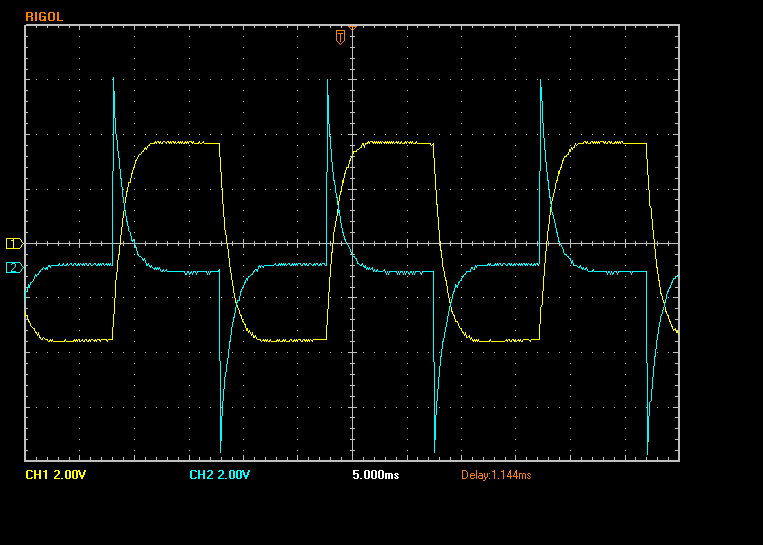
\includegraphics[scale=0.4]{winkler/Schaltung_1_Rechteck.png}}
\end{figure}




\subsection{RLC-Schwingkreis}


Hier wurde die Spannung über den Widerstand im RLC-Schwingkreis vermessen. Es gibt 3 mögliche Fälle
\begin{align*}
\begin{cases}
R^2\cdot C - 4\cdot L > 0 & 2 \text{ reelle Lösungen, Kriechfall} \\
R^2\cdot C - 4\cdot L = 0 & 1 \text{ reelle Lösung, aperiodischer Grenzfall} \\
R^2\cdot C - 4\cdot L < 0 & 2 \text{ konjugiert-komplexe Lösungen, Schwingfall}
\end{cases}
\end{align*}

\subsection{Schwingfall}


Im Schwingfall gilt
\begin{align*}
R^2\cdot C - 4\cdot L < 0
\end{align*}
Daraus folgt mit $R=200~\Omega$
\begin{align*}
R^2\cdot C < 4\cdot L \qquad\Longrightarrow\qquad \frac{R^2\cdot C}{4} < L \qquad\Longrightarrow\qquad 0.01 < L
\end{align*}
Die Induktivität der Spule muss also größer als $10~$mH sein. Um das zu erreichen wurde in beide Spulen der Metallkern eingesetzt. Grafik \ref{fig:schwing} zeigt den Verlauf der Spannung über den Widerstand.

\begin{figure}[H]
\caption{Spannungsverlauf über den Widerstand im RLC-Schwingkreis im Schwingfall. $f=50~$Hz, $R=1~$k$\Omega$, $C=1~\mu$F, beide Spulen ohne Kern.}
\label{fig:schwing}
{\centering
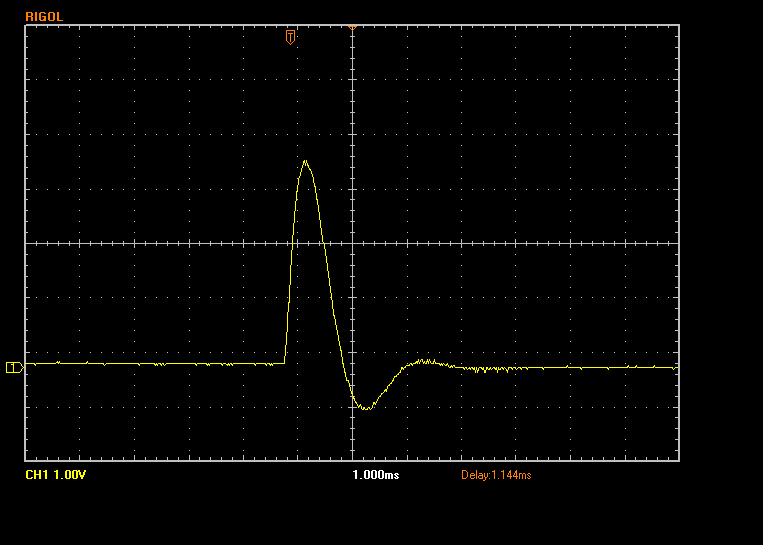
\includegraphics[scale=0.4]{winkler/schwingfall.png}}
\end{figure}


\subsection{Kriechfall}

Für den Kriechfall gilt
\begin{align*}
R^2\cdot C - 4\cdot L > 0
\end{align*}
Daraus folgt mit $R=1~$k$\Omega$
\begin{align*}
R^2\cdot C > 4\cdot L  \qquad\Longrightarrow\qquad \frac{R^2\cdot C}{4} > L \qquad\Longrightarrow\qquad 0.25 > L
\end{align*}
In diesem Fall wurde aus beiden Spulen der Kern entfernt. 

\begin{figure}[H]
\caption{Spannungsverlauf im Kriechfall.}
\label{fig:kriech}
{\centering
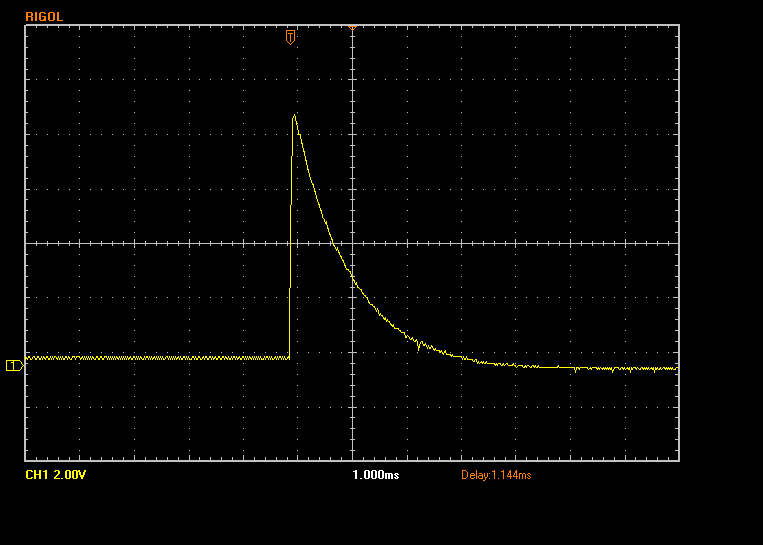
\includegraphics[scale=0.4]{winkler/kriechfall.png}}
\end{figure}



\subsection{Aperiodischer Grenzfall}

Im aperiodischen Grenzfall gilt
\begin{align*}
\frac{R^2\cdot C}{4} = L
\end{align*}
für $R=200~\Omega$. Daher gilt $L\approx 0.01$~H. Um diesen Fall zu erreichen wurde der Metallkern aus einer Spule entfernt, während der andere nur halb herausgezogen wurde.

\begin{figure}[H]
\caption{Spannungsverlauf im aperiodischen Grenzfall.}
\label{fig:kriech}
{\centering
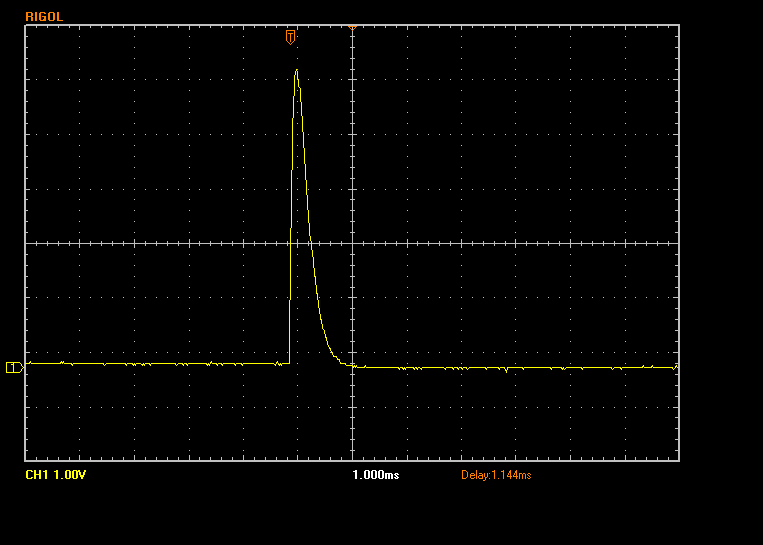
\includegraphics[scale=0.4]{winkler/aperiodischer_grenzfall.png}}
\end{figure}


\section{Zusammenfassung und Diskussion}



%\newpage 
\appendix
\section{Python Skript}



\definecolor{commentgreen}{RGB}{2,112,10}
\definecolor{eminence}{RGB}{108,48,130}
\definecolor{weborange}{RGB}{255,165,0}
\definecolor{frenchplum}{RGB}{129,20,83}

\lstdefinelanguage{python}{
    morekeywords={def, for, range, abs, return},
    otherkeywords={<-,->, |>, \%\{, \}, \{, \, (, )},
    sensitive=true,
    morecomment=[l]{\#},
    morecomment=[n]{/*}{*/},
    morecomment=[s][\color{purple}]{:}{\ },
    morestring=[s][\color{orange}]"",
    commentstyle=\color{commentgreen},
    keywordstyle=\color{eminence},
    stringstyle=\color{red},
	basicstyle=\ttfamily,
	breaklines,
	showstringspaces=false,
	frame=tb
}
\lstinputlisting[language=Python,captionpos=b, label=lst:test,caption={Sinus Auswertung von Schaltung 1}]{analyse/analyse_ges.py}

%\lstinputlisting[language=Python,captionpos=b, label=lst:test,caption={Bessel Auswertung}]{generate_numbers_bessel.py}


%\lstinputlisting[language=Python,captionpos=b, label=lst:test,caption={Zerstreuungslinse Auswertung}]{generate_numbers_zerstreuungslinse.py}


\begin{thebibliography}{9}
\bibitem{braun} \url{https://www.leifiphysik.de/elektrizitaetslehre/bewegte-ladungen-feldern/ausblick/braunsche-roehre}
\bibitem{youtube} \url{https://www.youtube.com/watch?v=TZQoyem7Jzo}
\bibitem{signale} \url{https://www.rahner-edu.de/grundlagen/signale-richtig-verstehen/schwingkreise/}
\bibitem{RLC} \url{https://itp.tugraz.at/wiki/index.php/RLC-Serienschwingkreis}
\bibitem{kondensator} \url{https://www.leifiphysik.de/elektrizitaetslehre/kondensator-kapazitaet/grundwissen/ein-und-ausschalten-von-rc-kreisen}
\bibitem{uniunterlagen} Unterlagen zum Versuch aus dem TeachCenter der TU Graz

\end{thebibliography}


\end{document}
